\documentclass[12pt]{article}

\usepackage[utf8]{inputenc}
\usepackage{datetime}
\usepackage{amsthm}
\usepackage{amsmath}
\usepackage{amssymb}
\usepackage{enumitem}
\usepackage[USenglish]{babel}
\usepackage{matlab-prettifier}
\usepackage{graphicx}
\usepackage[makeroom]{cancel}

\newcommand\independent{\protect\mathpalette{\protect\independenT}{\perp}}
\def\independenT#1#2{\mathrel{\rlap{$#1#2$}\mkern2mu{#1#2}}}

\newtheoremstyle{colon}{\topsep}{\topsep}{}{}{\bfseries}{:}{ }{}
\theoremstyle{colon}
\newtheorem{exercise}{Exercise}
\newtheorem*{answer}{Answer}

\title{ORFE 523: Conic and Convex Optimization \\ Homework 2}
\author{Zachary Hervieux-Moore}

\newdate{date}{09}{03}{2017}
\date{\displaydate{date}}

\begin{document}

\maketitle

\clearpage

\begin{exercise}
  Show that the convex hull of a set $S \subseteq \mathbb{R}^n$ is the intersection of all convex sets that contain $S$.
\end{exercise}

\begin{answer}
  The question asks to show that conv($S$) = $\bigcap_i A_i$ where the $A_i$'s are all the convex sets that contain $S$.

  Since conv($S$) is convex and contains $S$, by definition of intersection, we have $\bigcap_i A_i \subseteq$ conv($S$). Now, to show the other inclusion. By definition
  \begin{gather*}
    S \subseteq A_i \ \forall i \\
    \implies \text{conv}(S) \subseteq \text{conv}(A_i) \ \forall i \\
    \implies \text{conv}(S) \subseteq A_i \ \forall i \\
  \end{gather*}
  Where the last implication is because $A_i$ is convex. Since conv($S$) is a subset of $A_i$ for all $i$, we conclude that conv($S$) $\subseteq \bigcap_i A_i$ and so we have the equality conv($S$) = $\bigcap_i A_i$.
\end{answer}

\clearpage

\begin{exercise}
  Specify whether each of the following statements is true or false and provide either a proof or a counter-example depending on your answer. Let $S$ ne a set in $\mathbb{R}^n$.
  \begin{enumerate}[label=\roman*)]
    \item If $S$ is closed, then the convex hull of $S$ is closed.
    \item If $S$ is bounded, then the convex hull of $S$ is bounded.
    \item If $S$ is compact, then the convex hull of $S$ is compact. (You may want to use the following fact from analysis: the image of a compact set by a continuous mapping is compact.)
    \item The sum of two quasiconvex functions is quasiconvex.
    \item A convex homogeneous polynomial $p(x)$ of degree $d \geq 2$ is nonnegative. (Recall that a polynomial is homogeneous of degree $d$ if all of its monomials have degree exactly $d$, and that $p(x)$ is nonnegative if $p(x) \geq 0$ for all $x \in \mathbb{R}^n$.)
    \item A quadratic function $f(x) = x^T Q x + b^T x + c$ is convex if and only if it is quasiconvex. (You can use the fact that $f$ is convex if and only if $Q \succeq 0$ if you need to.)
  \end{enumerate}
\end{exercise}

\begin{answer}
  \leavevmode
  \begin{enumerate}[label=\roman*)]
    \item This is false. Consider the line created from $e^x$ from $(-\infty, 0]$. This is closed as it is a continuous mapping of a closed set. However, the convex hull is open as one get get arbitrarily close to the the points on the line $(x, 1)$ where $x \in (-\infty, 0]$ but cannot achieve it.
      \bigskip

    \item This is true. Suppose $x \in S \subset \mathbb{R}^d$. Then, for each component, we have $C_1 \leq x_i \leq C_2$ for $i \in \{1, \mathellipsis, d\}$. Then, by Caratheodory, we can express any point in the convex hull with $d+1$ points in $S$ and $\lambda_i \in (0,1)$ with $\sum \lambda_i = 1$. We have
      \begin{gather*}
        \sum_{i=1}^{d+1} \lambda_i x^i \in \text{conv}(S)
      \end{gather*}
      However, in each compenent, we have
      \begin{gather*}
        \sum_{i=1}^{d+1} \lambda_i C_1 \leq \sum_{i=1}^{d+1} \lambda_i x_j^i \leq \sum_{i=1}^{d+1} \lambda_i C_2 \ \forall j \in \{ 1, \mathellipsis, d \} \\
        C_1 \sum_{i=1}^{d+1} \lambda_i \leq \sum_{i=1}^{d+1} \lambda_i x_j^i \leq C_2 \sum_{i=1}^{d+1} \lambda_i \ \forall j \in \{ 1, \mathellipsis, d \} \\
        C_1 \leq \sum_{i=1}^{d+1} \lambda_i x_j^i \leq C_2 \ \forall j \in \{ 1, \mathellipsis, d \}
      \end{gather*}
      Thus, any point in the convex hull is bounded and so the convex hull is bounded.

    \item We shall apply the Bolzano-Weierstrass theorem that says that every bounded sequence has a convergent subsequence. Then pick a sequence $(x^n)_n$ that converges to a limit point in the convex hull of $S$. By Caratheodory, we can represent this point as a convex combination of $d+1$ points in $S$. So,
      \begin{gather*}
        \sum_{i=1}^{d+1} \lambda_i y_i^n = x^n \in \text{conv}(S), \ y_i^n \in S
      \end{gather*}
      Now, we show that the limit is also in conv($S$). By Bolzano-Weierstrass, pick a subsequence that converges for $y_1$. Call this sequence $n_1$. Now, from $n_1$, pick a convergent subsequence that converges for $y_2$, call it $n_2$. Do this for each $y_i$ until we have $n_{d+1}$. Thus, we have
      \begin{gather*}
        \sum_{i=1}^{d+1} \lambda_i y_i^{n_{d+1}} = x^{n_{d+1}} \in \text{conv}(S)
      \end{gather*}
      Now, we take the limit on both sides. Since the left hand side converges, the right hand side must as well.
      \begin{gather*}
        \lim_{n \rightarrow \infty} \sum_{i=1}^{d+1} \lambda_i y_i^{n_{d+1}} = \lim_{n \rightarrow \infty} x^{n_{d+1}} \\
        \sum_{i=1}^{d+1} \lambda_i \bar{y}_i = \bar{x} \in \text{conv}(S)
      \end{gather*}
      Where $\bar{y}_i \in S$ since $S$ is compact. Thus, all limit points are contained in conv($S$) and so conv($S$) is closed. Boundedness comes from part ii).

    \item The sum of two quasiconvex functions is not quasiconvex. Consider $f(x) = \sqrt{\lvert x - 1 \rvert}$ and $g(x) = \sqrt{\lvert x + 1 \rvert}$. Now consider the sublevel set $S_{1.5}$ of $f(x) = g(x)$. Then $x = 1$ and $x = -1$ both are equal to $\sqrt{2} \leq 1.5$ and so are in $S_{1.5}$. However, $x = 0$ which equals $2 \sqrt{2}> 1.5$ and so not in $S_{1.5}$. But $0 = \frac{1}{2} -1 + \frac{1}{2} 1$ and so $S_{1.5}$ is not convex.

    \item First note that $p(0) = 0$ for all homogeneous polynomial of $d \geq 2$. Now suppose there exists a point $x$ such that $p(x) < 0$. Then consider the convex combination of 0 and $x$ with $\lambda = 1/2$. By convexity we have
      \begin{gather*}
        p(\frac{1}{2} x) = p(\frac{1}{2}0 + \frac{1}{2}x) \leq \frac{1}{2} p(0) + \frac{1}{2} p(x) = \frac{1}{2} p(x)
      \end{gather*}
      However, note that for homogeneous polynomials of degree $d$, we have the following property
      \begin{gather*}
        p(\lambda x) = \lambda^d p(x) \ \forall \lambda \in \mathbb{R}
      \end{gather*}
      Thus,
      \begin{gather*}
        p(\frac{1}{2} x) = \frac{1}{2^d} p(x)
      \end{gather*}
      Which we showed that
      \begin{gather*}
        p(\frac{1}{2} x) = \frac{1}{2^d} p(x) \leq \frac{1}{2} p(x)
      \end{gather*}
      However, since $p(x) < 0$ and $d \geq 2$, we must have
      \begin{gather*}
        \frac{1}{2^d} p(x) > \frac{1}{2} p(x)
      \end{gather*}
      Which is a contradiction and so we must not have $p(x) < 0$ for some $x$. We conclude that $p(x) \geq 0$.

    \item Suppose $f(x)$ is convex. Then
      \begin{gather*}
        f(\lambda x + (1-\lambda)y ) \leq \lambda f(x) + (1-\lambda) f(y)
      \end{gather*}
      Now, suppose that $f(x)$ and $f(y) \leq \alpha$. Then by the above
      \begin{gather*}
        \lambda f(x) + (1-\lambda) f(y) \leq \lambda \alpha + (1-\lambda) \alpha = \alpha
      \end{gather*}
      Therefore, if $f(x)$ and $f(y) \leq \alpha$,
      \begin{gather*}
        f(\lambda x + (1-\lambda)y ) \leq \alpha
      \end{gather*}
      Thus, convexity implies quasiconvexity. Now suppose that $f(x)$ is not convex. Then we have that $Q \cancel{\succeq} 0$ since $f(x)$ is convex iff $Q \succeq 0$. That is, there exists an eigenvector with eigenvalue $\lambda < 0$. Denote this eigenvector by $u$. Then we have
      \begin{gather*}
        f(a u) = a^2 \lambda \lVert u \rVert^2 + a b^T u + c
      \end{gather*}
      Maximizing this, we get
      \begin{gather*}
        \arg\max_a f(a u) = a^* =  - \frac{b^T u}{2 \lambda \lVert u \rVert^2 } \\
      \end{gather*}
      This is clearly a maximum since it is a univariable quadratic with the leading term negative (since $\lambda < 0$). Thus, we have that
      \begin{gather*}
        f(a^* u) > f((a^* + 1) u) = f((a^* - 1) u)
      \end{gather*}
      Thus it is not quasiconvex because picking $\alpha = f((a^* + 1) u)$. We have that $(a^* + 1) u$ and $(a^* - 1) u \in S_\alpha$. However, the convex combination of $\frac{1}{2}(a^* + 1) u + \frac{1}{2}(a^* - 1) u$ yields $f(a^* u) > \alpha$.
  \end{enumerate}
\end{answer}

\clearpage

\begin{exercise}
  Use Matlab to find the solution to the following problem. $T_i \geq 0$, $A_i \geq 0$, and $T_i + A_i = 1$, $i \in \{ 1, \mathellipsis, 24 \}$. We also have the following constraints
  \begin{gather*}
    A_1 + \mathellipsis + A_i \leq a \max (0, T_1 + \mathellipsis + T_i - b) \ \forall i \\
    s_i = (1-\theta)s_{i-1} + \theta (\alpha T_i + \beta A_i) \ \forall i
  \end{gather*}
  The constants we have are $a = 2$, $b = 3$. We wish to maximize $s_1 + \mathellipsis + s_{24}$ for the following 3 sets parameters
  \begin{center}
    \begin{tabular}{|c|c|c|c|}
      \cline{2-4}
      \multicolumn{1}{c|}{}
      & Group 1 & Group 2 & Group 3 \\
      \hline
      $\theta$ & 0.05 & 0.1 & 0.3 \\
      \hline
      $\alpha$ & -0.1 & 0.8 & -0.3 \\
      \hline
      $\beta$ & 1.4 & -0.3 & 0.7 \\
      \hline
    \end{tabular}
  \end{center}
  As well, find the $s_i$'s that minimize the CES of all three groups. Give your plots for the $s_i$'s of the 3 groups for all 4 plans and the value of $T_i$.
\end{exercise}

\begin{answer}
  The filled out table is below. The code is appended at the end. Figure 1 shows the different CES scores for plan 1, Figure 2 for plan 2, Figure 3 for plan 3, and Figure 4 for plan 4. Note that we have two solutions that are the same. It's just chance that they are the same. Essentially, $\theta$ is not great enough to encourage either Group 1 or Group 3 to learn more theory in the beginning so that they can have lectures with mostly application. If $\alpha \geq \beta$, then all learning is done in theory since the students gain more from theory always. Thus, $T_i = 1$ for all $i$. Which is what we see for Group 2.
  \begin{center}
    \begin{tabular}{|c|c|c|c|}
      \cline{2-4}
      \multicolumn{1}{c|}{}
      & Group 1 & Group 2 & Group 3 \\
      \hline
      Plan 1 & 7.42 & 3.05 & 5.95 \\
      \hline
      Plan 2 & -1.05 & 12.57 & -6.50 \\
      \hline
      Plan 3 & 7.42 & 3.05 & 5.95 \\
      \hline
      Plan 4 & 5.19 & 4.98 & 4.98 \\
      \hline
    \end{tabular}
  \end{center}

  \begin{figure}[ht]
    \caption{Plots for maximization of CES for group 1}
    \centering
      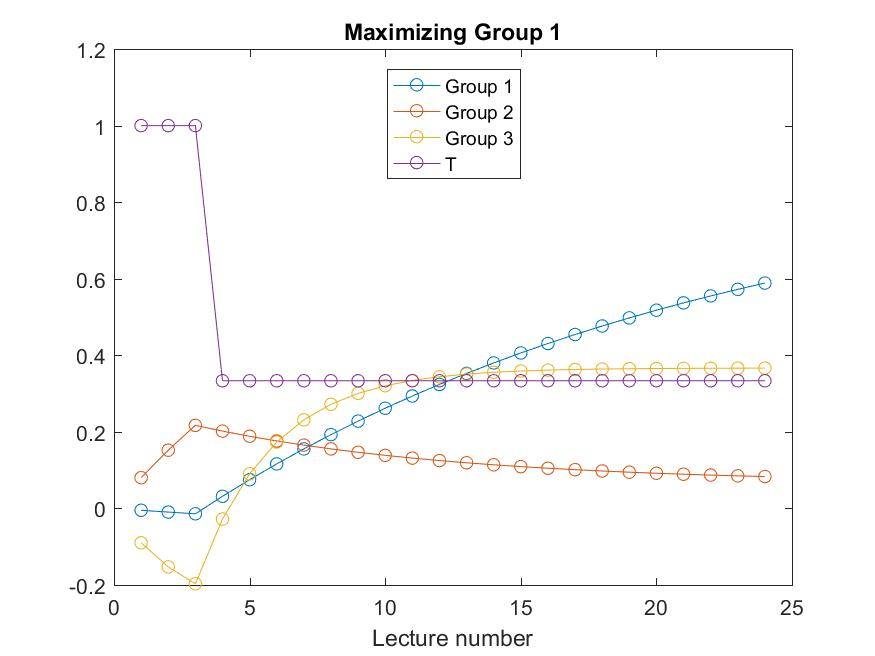
\includegraphics[width=0.8\textwidth]{group1.jpg}
  \end{figure}

  \begin{figure}[ht]
    \caption{Plots for maximization of CES for group 2}
    \centering
      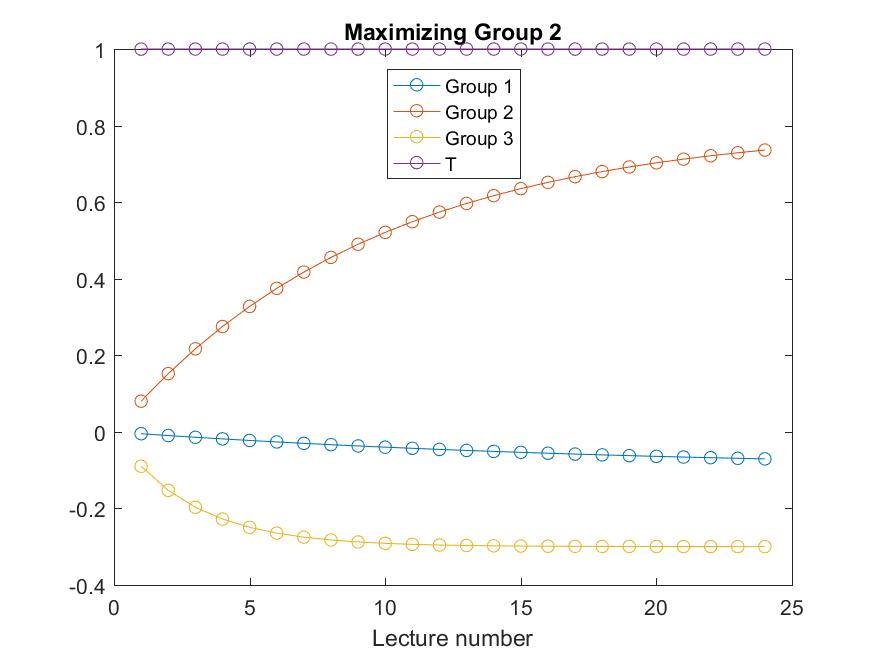
\includegraphics[width=0.8\textwidth]{group2.jpg}
  \end{figure}

  \begin{figure}[ht]
    \caption{Plots for maximization of CES for group 3}
    \centering
      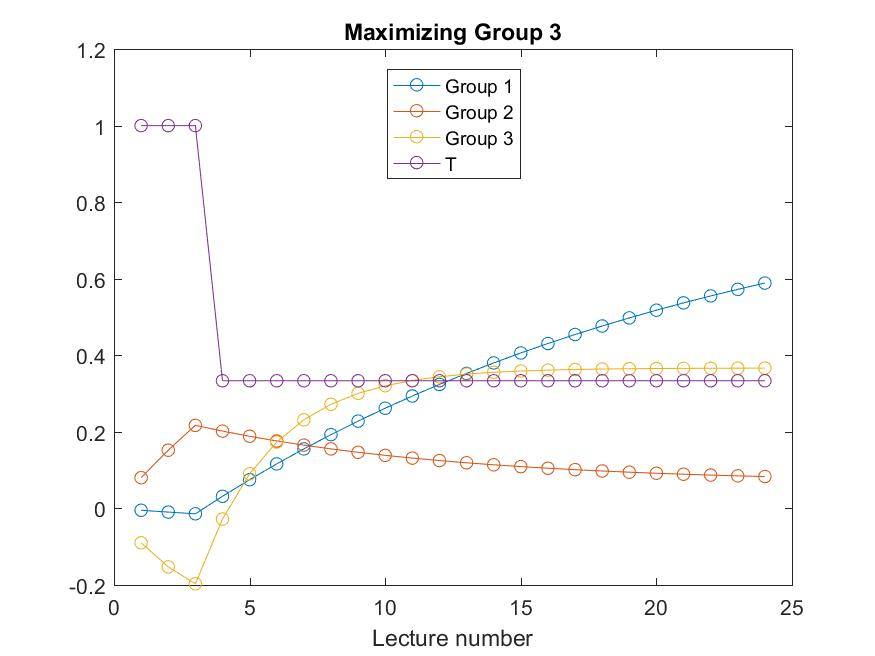
\includegraphics[width=0.8\textwidth]{group3.jpg}
  \end{figure}

  \begin{figure}[ht]
    \caption{Plots for maximization of min CES for all groups}
    \centering
      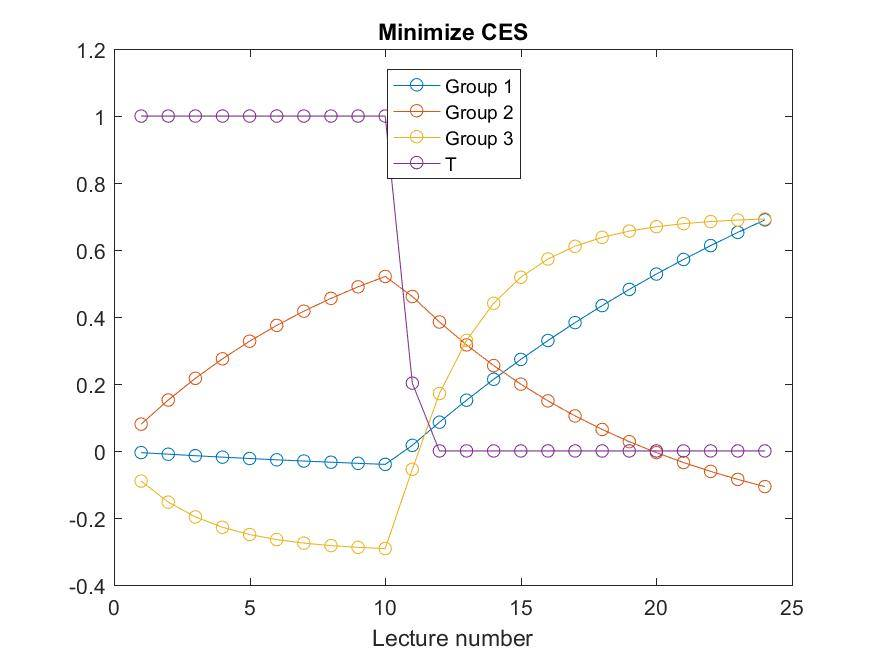
\includegraphics[width=0.8\textwidth]{minCES.jpg}
  \end{figure}

  \clearpage

  \textbf{Code Appendix}

  \begin{lstlisting}[style=Matlab-editor, basicstyle=\scriptsize]
    clear;
    clc;

    a = 2;
    b = 3;
    n = 24;

    cvx_begin
        variable s(n);
        variable T(n);
        variable A(n);
        % Vary these according to the group
        theta = 0.3;
        alpha = -0.3;
        beta = 0.7;

        maximize(sum(s));

        subject to

        % dynamics
        s(1) == theta*(alpha*T(1) + beta*A(1));

        % max(0, sum(T(1:i)-b,0) is 0 for the first b entries
        % need to do this so that the RHS is affine
        for i = 1:b
          A(i) <= 0;
        end
        for i = b+1:n
          sum(A(1:i)) <= a*(sum(T(1:i))-b);
        end

        A(1) >= 0;
        T(1) >= 0;
        A(1) + T(1) == 1;
        for i = 2:n
            s(i) == (1-theta)*s(i-1) + theta*(alpha*T(i) + beta*A(i));
            T(i) >= 0;
            A(i) >= 0;
            A(i)+T(i) == 1;
        end
    cvx_end

    % Calculate CES for the three groups

    % CES of first group
    theta = 0.05;
    alpha = -0.1;
    beta = 1.4;
    s_1(1) = theta*(alpha*T(1) + beta*A(1));
    for i = 2:n
        s_1(i) = (1-theta)*s_1(i-1) + theta*(alpha*T(i) + beta*A(i));
    end

    disp('CES of Group 1')
    sum(s_1)

    % CES of first group
    theta = 0.1;
    alpha = 0.8;
    beta = -0.3;
    s_2(1) = theta*(alpha*T(1) + beta*A(1));
    for i = 2:n
        s_2(i) = (1-theta)*s_2(i-1) + theta*(alpha*T(i) + beta*A(i));
    end

    disp('CES of Group 2')
    sum(s_2)

    % CES of third group
    theta = 0.3;
    alpha = -0.3;
    beta = 0.7;
    s_3(1) = theta*(alpha*T(1) + beta*A(1));
    for i = 2:n
        s_3(i) = (1-theta)*s_3(i-1) + theta*(alpha*T(i) + beta*A(i));
    end

    disp('CES of Group 3')
    sum(s_3)

    % plot graphs, change titles accordingly
    figure1 = figure
    plot(1:n, s_1, '-o', 1:n, s_2, '-o', 1:n, s_3, '-o', 1:n, T, '-o')
    title('Maximizing Group 3')
    xlabel('Lecture number')
    legend('Group 1','Group 2','Group 3','T','location','north')
    saveas(figure1,'group3.jpg')

    % Plan 4, minimize CES
    cvx_begin
        variable s_1(n);
        variable s_2(n);
        variable s_3(n);
        variable T(n);
        variable A(n);

        % Parameters for the 3 groups
        theta_1 = 0.05;
        alpha_1 = -0.1;
        beta_1 = 1.4;
        theta_2 = 0.1;
        alpha_2 = 0.8;
        beta_2 = -0.3;
        theta_3 = 0.3;
        alpha_3 = -0.3;
        beta_3 = 0.7;

        maximize min([sum(s_1),sum(s_2),sum(s_3)]);

        subject to

        % dynamics
        s_1(1) == theta_1*(alpha_1*T(1) + beta_1*A(1));
        s_2(1) == theta_2*(alpha_2*T(1) + beta_2*A(1));
        s_3(1) == theta_3*(alpha_3*T(1) + beta_3*A(1));

        % max(0, sum(T(1:i)-b,0) is 0 for the first b entries
        % need to do this so that the RHS is affine
        for i = 1:b
          A(i) <= 0;
        end
        for i = b+1:n
          sum(A(1:i)) <= a*(sum(T(1:i))-b);
        end

        A(1) >= 0;
        T(1) >= 0;
        A(1) + T(1) == 1;
        for i = 2:n
            s_1(i) == (1-theta_1)*s_1(i-1) + theta_1*(alpha_1*T(i) + beta_1*A(i));
            s_2(i) == (1-theta_2)*s_2(i-1) + theta_2*(alpha_2*T(i) + beta_2*A(i));
            s_3(i) == (1-theta_3)*s_3(i-1) + theta_3*(alpha_3*T(i) + beta_3*A(i));
            T(i) >= 0;
            A(i) >= 0;
            A(i)+T(i) == 1;
        end
    cvx_end

    % Show CES

    disp('CES of Group 1')
    sum(s_1)

    disp('CES of Group 2')
    sum(s_2)

    disp('CES of Group 3')
    sum(s_3)

    figure2 = figure
    plot(1:n, s_1, '-o', 1:n, s_2, '-o', 1:n, s_3, '-o', 1:n, T, '-o')
    title('Minimize CES')
    xlabel('Lecture number')
    legend('Group 1','Group 2','Group 3','T','location','north')
    saveas(figure2,'minCES.jpg')
  \end{lstlisting}
\end{answer}

\clearpage

\begin{exercise}
  Consider the LP
  \begin{gather*}
    \min_x c^T x \\
    \text{s.t. } Ax = b \\
    x \geq 0
  \end{gather*}
  where $A$ is $m \times n$, all data (i.e., $A$, $b$, $c$) is rational, and the feasible set is non-empty and bounded. Suppose you have a black box that, when given any LP with a non-empty and bounded feasible set and rational data, outputs its optimal value. How could you make a polynomial number of calls to this black box to decide if the optimal solution to the above LP is unique?
\end{exercise}

\begin{answer}
  The algorithm first goes as follows. Give it the original problem and record the optimal value as $f^*$. This is rational because $x^*$ must satisfy $A x^* = b$ and so $x^*$ must be rational if $A$ and $b$ are rational (finite multiplications of rationals). Thus, $f^*$ is rational since $c^T x^*$ is rational for the same reason. Now to check uniqueness, write out two new LP's as
  \begin{gather*}
    \min x_i \\
    \text{s.t.} A x \leq b \\
      c^T x = f^* \\
      x \geq 0
  \end{gather*}
  and
  \begin{gather*}
    \max x_i \\
    \text{s.t.} A x \leq b \\
      c^T x = f^* \\
      x \geq 0
  \end{gather*}
  Clearly, these are both feasible and non-empty because $x^*$ which satisfied the original problem is feasible. It is also bounded since the first problem is bounded and we are adding a constraint. Now, the purpose here is to check if there is a difference in the $i^{th}$ coordinate. The idea is that if there are multiple optimal solutions, they must differ in at least one coordinate. If these optimal values do not match, it means there is one optimal solution with a different $x_i$ coordinate. Hence, we repeat the above except switch the objective to go through all the coordinates $x_1, x_2, \mathellipsis, x_n$. If both the min and max match for each coordinate, then the solution is unique. This is $2n + 1$ calls which is polynomial time.
\end{answer}

\clearpage

\begin{exercise}
  The distance between two sets $S_1$ and $S_2$ is the closest distance between any two points one taken from each set.
  \begin{enumerate}[label=\arabic*)]
    \item Consider an elliptic cylinder $S_1$, given by
      \begin{gather*}
        S_1 = \left\{ (x_1, x_2, x_3) \in \mathbb{R}^3 :
        \begin{pmatrix}
          1 & x_1 & x_2 \\
          x_1 & 1 & 0.5 \\
          x_2 & 0.5 & 1
        \end{pmatrix} \succeq 0, 0 \leq x_3 \leq 1 \right\}
      \end{gather*}
      and an ellipsoid $S_2$, given by $S_2 = \{ x \in \mathbb{R}^3 : x^T Q x + b^T x + c \leq 1 \}$, where
      \begin{gather*}
        Q = \begin{pmatrix}
          4/9 & 0 & 0 \\
          0 & 4 & 0 \\
          0 & 0 & 1/4
        \end{pmatrix}, b = \begin{pmatrix}
          16/9 & 16 & 1
        \end{pmatrix}^T, c = 169/9
      \end{gather*}
      Formulate the problem of finding the distance between $S_1$ and $S_2$ as a convex optimization problem. Use CVX to find this distance and report the value.

    \item Using the commands \texttt{hold on} and \texttt{plot3}, plot the MATLAB figure (given in \texttt{distance\_computation.fig}) the two points that achieve the minimum distance computed in the previous question as well as a line segment connecting them.

    \item Recall that a point $x$ is an \textit{extreme point} of a convex set $S$ if it is in $S$ and cannot be written as a convex combination of two other points in $S$. In other words, there does not exist $y, z \in S$, $y \neq x$, $z \neq x$, and $\lambda \in (0,1)$ such that $\lambda y + (1-\lambda)z = x$.

      A student who hasn't taken ORF523 claims that for any two bounded and closed convex sets $S_1$ and $S_2$ which do not intersect, there exists an extreme point in $S_1$ or in $S_2$ where the minimum distance between $S_1$ and $S_2$ is achieved. Prove the student wrong. (A correct picture is enough).
  \end{enumerate}
\end{exercise}

\begin{answer}
  \leavevmode
  \begin{enumerate}[label=\arabic*)]
    \item The minimum distance between the ellipse and the cylinder is 1.088. The code used to generate this is shown below. The CVX code is different than the convex problem but equivalent in optimal solution $x^*$. You have to take the square root of the convex optimal value to retrieve the SDP value. The convex problem of this optimization can be written as
      \begin{gather*}
        \min \lVert x_1 - x_2 \rVert_2^2 \\
        \text{s.t. } 0 \leq x_{1_3} \leq 1 \\
        x_2^T \begin{bmatrix}
          4/9 & 0 & 0 \\
          0 & 4 & 0 \\
          0 & 0 & 1/4
        \end{bmatrix} x_2 + \begin{bmatrix}
          16/9 & 16 & 1
        \end{bmatrix} x_2 + 160/9 \leq 0 \\
        1 - x_{1_1}^2 \geq 0 \\
        0.75 - x_{1_1}^2 + x_{1_1} x_{1_2} - x_{1_2}^2 \geq 0
      \end{gather*}
      Where the last two constraints are the conditions for the ellipse to be psd by Sylvester's criterion. Note that the inequalities are convex once they are on the appropriate side of the inequality. The first inequality is linear and hence convex. The second is a quadratic with a positive definite $Q$ hence convex. The third is again clearly a convex quadratic. The last inequality is convex since the Hessian is positive definite. Finally, the objective is convex since we squared it the 2-norm.

      \textbf{Code Appendix}

      \begin{lstlisting}[style=Matlab-editor, basicstyle=\scriptsize]
        clear;
        clc;

        cvx_begin
            % x_1 in cylinder, x_2 in ellipsoid
            variable x_1(3);
            variable x_2(3);

            minimize norm(x_1 - x_2)

            [1, x_1(1), x_1(2); x_1(1), 1, 0.5; x_1(2), 0.5, 1] == semidefinite(3)
            0 <= x_1(3) <= 1
            x_2'*[4/9,0,0;0,4,0;0,0,1/4]*x_2 + [16/9, 16, 1]*x_2 + 169/9 <= 1

        cvx_end

        figure1 = openfig('distance_computation.fig')
        hold on
        plot3([x_1(1),x_2(1)],[x_1(2),x_2(2)],[x_1(3),x_2(3)])
        saveas(figure1,'question5.jpg')
      \end{lstlisting}

    \item Below is the image with the line between the two points. If you had the figure in MATLAB, it's easy to see that the line is perpendicular to the ellipsoid which is what you would expect. The two points are $x_1 = (-0.756, -0.945, 0)^T \in S_1$ and $x_2 = (-1.196, -1.822, -0.4701)^T \in S_2$.
      \begin{figure}[ht]
        \caption{3D Plot of the line}
        \centering
          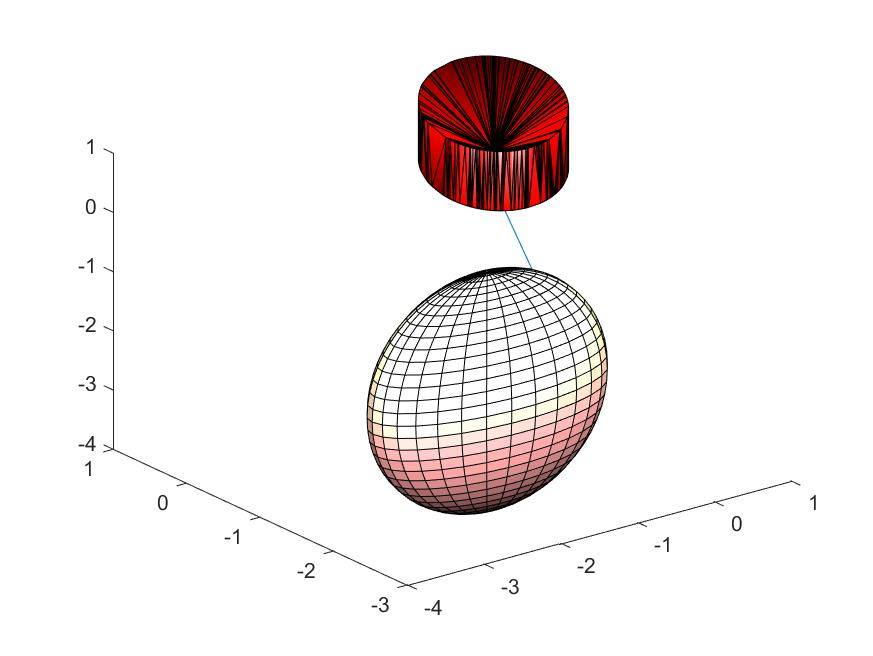
\includegraphics[width=\textwidth]{question5.jpg}
      \end{figure}

    \item Consider two lines in $\mathbb{R}^3$. One goes from $(-1,0,0)$ to $(1,0,0)$. The other goes from $(0, -1, 1)$ to $(0,1,1)$. These are both closed, bounded, and convex. The minimum distance occurs between $(0,0,0)$ and $(0,0,1)$ for a minimum distance of 1. This is the minimum because the line between $(0,0,0)$ and $(0,0,1)$ is orthogonal to both lines. However, neither of these points are extreme points. Hence, we showed what we wished to show.
  \end{enumerate}
\end{answer}

\end{document}